


%----------------------------------------------------------------------------------------

\newpage

%\chapter{Thematic Developments}{Développements Thématiques} % Chapter title
\chapter{Développements Thématiques}

\label{app:thematic} % For referencing the chapter elsewhere, use \autoref{ch:name} 

%----------------------------------------------------------------------------------------








%----------------------------------------------------------------------------------------


\section[Bridges between Economics and Geography][Ponts entre Géographie et Economie]{Bridges between Economics and Geography : lessons from modeling perspectives}{Ponts entre Géographie et Economie : leçons des perspectives de modélisation}

\label{app:sec:ecogeo}














\stars

\newpage



%----------------------------------------------------------------------------------------



\section{An Interdisciplinary Approach to Morphogenesis}{An Interdisciplinary Approach to Morphogenesis}

\label{app:sec:morphogenesis} % For referencing the chapter elsewhere, use \autoref{ch:name} 

%----------------------------------------------------------------------------------------

include quant epistemo analysis of morphogenesis papaers

%\textit{This Appendix was submitted as an Essay Paper with C. Antelope (U. California), L. Hubatsch (F. Crick Institute) and J.M. Serna (Université Paris 7), as : }
%\noindent Antelope, C., Hubatsch, L., Raimbault, J., and Serna, J. M. (2016). An interdisciplinary approach to morphogenesis. \textit{Forthcoming in Proceedings of Santa Fe Institute CSSS 2016.}









\stars

\newpage




%----------------------------------------------------------------------------------------


\section{Optimal design of transportation network infrastructure}{Design optimal d'infrastructures de transport}

\label{app:sec:biological}





%%%%%%%%%%%%%%%%%%%%%%
\begin{figure}
%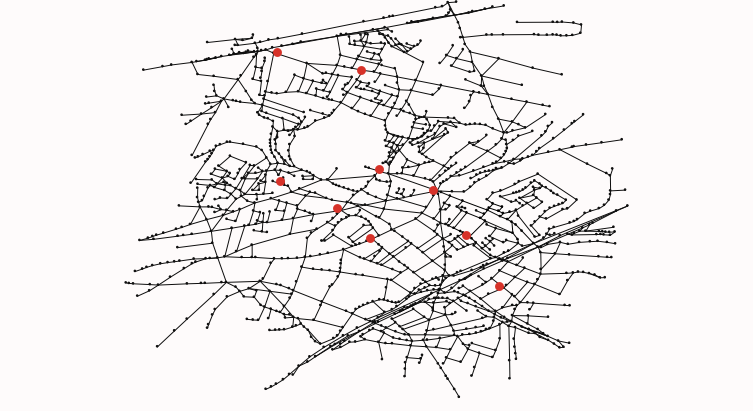
\includegraphics[width=0.45\textwidth]{Figures/NetworkGrowth/tick1}
%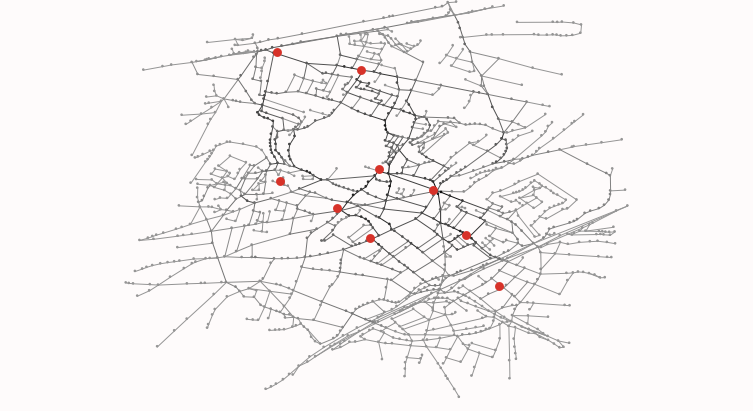
\includegraphics[width=0.45\textwidth]{Figures/NetworkGrowth/tick20}\\
%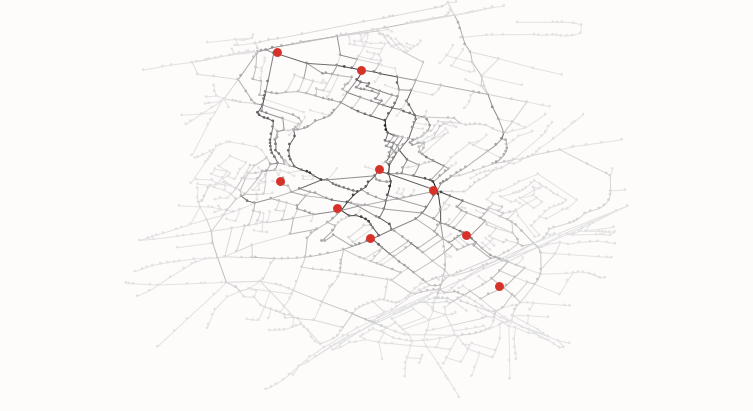
\includegraphics[width=0.45\textwidth]{Figures/NetworkGrowth/tick50}
%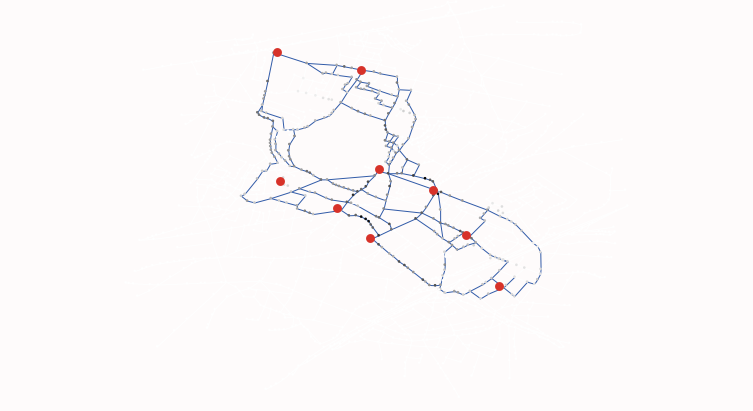
\includegraphics[width=0.45\textwidth]{Figures/NetworkGrowth/reseauFinal}
\caption[Biological Network Growth][Croissance de réseau biologique]{Example of the application of the slime mould network generation model to the computation of an optimal public transportation network design.}{\comment{(Florent) source ?}}
\label{fig:slimemould}
\end{figure}
%%%%%%%%%%%%%%%%%%%%%%%

